\documentclass[border=0.2cm]{standalone}
 
% More defined colors
\usepackage[dvipsnames]{xcolor}
\usepackage{tikz}
\usetikzlibrary{positioning}
\usepackage{xstring}
\usetikzlibrary{arrows.meta,shapes.arrows}

\begin{document}
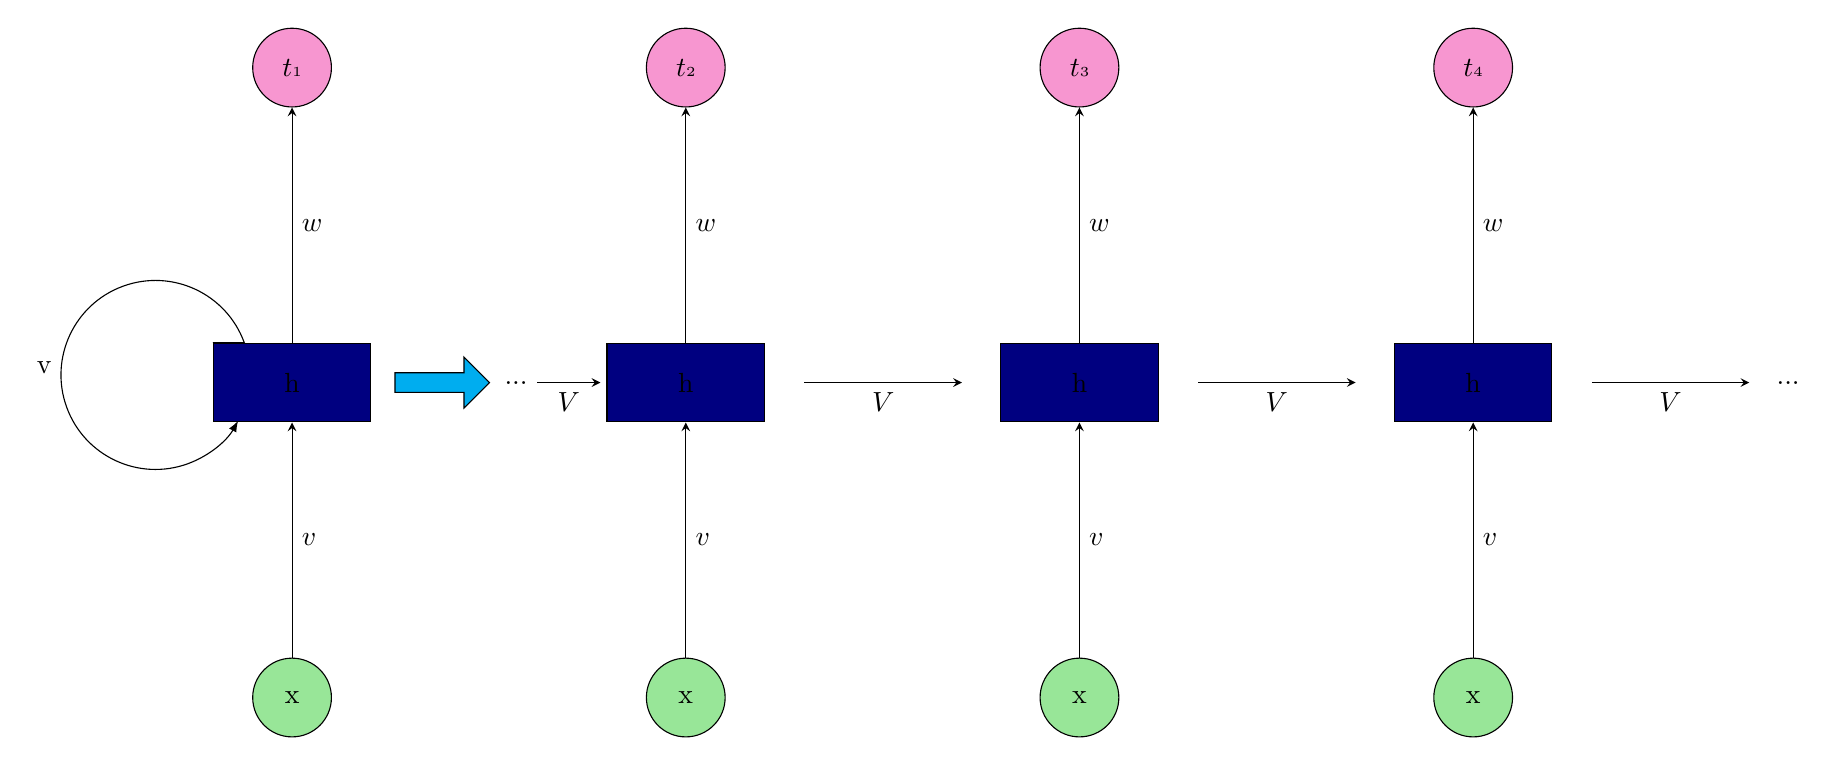
\begin{tikzpicture}

\newcommand{\numlayerA}{4}
\newcommand{\nodedis}{8}

at (\i*4,0) \foreach \i in {1,...,\numlayerA}
{
    \node [draw, fill=NavyBlue, minimum width=2cm, minimum height=1cm] (controller\i) at (\i*5,0) {h};
    \node [draw, circle, minimum size=1cm, fill=Rhodamine!50, above of=controller\i, node distance=4cm ] (circlea\i) { $t$\tiny \i };
    \node [draw, circle, minimum size=1cm, fill=LimeGreen!50, below of=controller\i, node distance=4cm ] (circleb\i) {x};
    \draw [stealth-] (circlea\i.south) -- (controller\i.north) node[midway,right] {$w$};
    \draw [-stealth] (circleb\i.north) -- (controller\i.south) node[midway,right] {$v$};
    \IfEq{\i}{1}%
     {\node[draw, single arrow, fill=cyan, minimum height=12mm, minimum width=.1cm, single arrow head extend=2mm, anchor=west] at (6.3,0) (arrowh) {};
     \node[right of=arrowh ] (dot\i) {...};
     \draw [-stealth] (dot\i.east) -- node[below] (arrow\i) {$V$} ++(.8,0);
     }
     { \draw [-stealth] (controller\i.east)+(.5cm,0) -- node[below] (arrow\i) {$V$} ++(2.5,0); }
}

\draw[-latex] (controller1.north west) -- ++ (.4,0) arc[start angle=20, end angle=331, x radius=1.2cm, y radius =1.2cm] node[midway, left] {v};

\node[right of=controller\numlayerA, node distance=4cm] {...};

\end{tikzpicture}
\end{document}